\documentclass[12pt,a4paper]{article}

\usepackage[left=3cm, right=3cm, top=2.5cm, bottom=2.5cm, headheight=38.40865pt]{geometry} % Adjusted headheight
\usepackage{setspace}
\usepackage{amsmath}
\usepackage{tikz}
\usepackage{pgfplotstable}
\usepackage{titlesec}
\usepackage{bm}
\usepackage{tcolorbox}
\tcbuselibrary{skins}
\usepackage{empheq}
\usepackage{booktabs}
\usepackage{caption}
\usepackage{hyperref}
\usepackage{fancyhdr}
\usepackage{float}
\usepackage{silence}
\usepackage{multirow}
\usepackage{verbatim}
\usepackage{listings}
\WarningFilter{caption}{The option `hypcap=true' will be ignored}
\WarningFilter{latex}{Underfull \hbox}
\hypersetup{
    colorlinks=true,
    linkcolor=black,
    filecolor=magenta,      
    urlcolor=cyan,
    pdfpagemode=FullScreen,
    }
\usepackage{graphicx}
\graphicspath{ {./images/} }

\pgfplotsset{compat=1.18}

\titleformat{\section}{\Large\bfseries}{\thesection}{1em}{}
\titleformat{\subsection}{\large\bfseries}{\thesubsection}{1em}{}

% Define colors for syntax highlighting
\definecolor{mygray}{rgb}{0.5,0.5,0.5}
\definecolor{mygreen}{rgb}{0,0.6,0}
\definecolor{myorange}{rgb}{0.8,0.4,0}

\lstset{
    language=C,
    basicstyle=\footnotesize\ttfamily,
    numbers=left,
    numberstyle=\tiny\color{mygray},
    commentstyle=\itshape\color{mygreen},
    keywordstyle=\bfseries\color{blue},
    stringstyle=\color{myorange},
    showstringspaces=false,
    frame=single,
    breaklines=true,
    breakatwhitespace=true,
    tabsize=4,
    captionpos=b,
    morekeywords={include, define},
    emph={int, char, if, else, for, while},
    emphstyle=\color{purple},
    escapeinside={(*@}{@*)},
}

\title{Interférences et diffraction de la lumière}
\author{Liviu Arsenescu, Cătălin Bozan}
\date{28.05.2024}

\pagestyle{fancy}
\fancyhf{}
\rhead{
\includegraphics[width=4cm]{hearclogo.png}}
\lhead{\thepage}
\setlength{\headsep}{30pt}

\begin{document}
    \pagenumbering{gobble}
    \begin{titlepage}
        \begin{center}
            \vspace*{\fill}
            \Huge \textbf{Client SMTP in C} \\
            \Large Instructions and documentations \\
            \begin{figure}[h]
                \centering
                
\includegraphics[width=7cm]{hearclogo.png}
            \end{figure}
            \vspace{\fill}
            \Large Liviu Arsenescu \\
            16.06.2024

            \vspace*{\fill}
        \end{center}
    \end{titlepage}

    \tableofcontents
    \pagenumbering{arabic}
    \newpage

    \section{Introduction}
    Welcome to the documentation for the Simple SMTP Client, a project developed for the Networking course at HE-Arc Ingénierie. This project showcases the practical application of networking concepts by implementing a basic SMTP client, designed to facilitate the understanding of email protocols and client-server communication.
    \section{Client usage}
    \subsection{Synopsis}
    \begin{verbatim}
        bin/client_smtp
            <sender email>
            <subject>
            <message file>
            <mail server>
            <reciever email>
            [<port>]
    \end{verbatim}
    \subsection{Description}
    \verb|<sender email>| - Email address of the sender. \\
    \verb|<subject>| - Subject of the email. \\
    \verb|<message file>| - Path to the file containing the message. \\
    \verb|<mail server>| - Address of the mail server. \\
    \verb|<reciever email>| - Email address of the reciever. \\
    \verb|[<port>]| - (optional) Port number of the mail server. Default is 25.
    \subsection{Example}
    \begin{verbatim}
        bin/client_smtp
            liviu-andrei.arsenescu@he-arc.ch
            "Some Subject"
            mail_body.txt
            smtp.alphanet.ch
            liviu-andrei.arsenescu@he-arc.ch
            587
    \end{verbatim}
    \subsection{Compile the program}
    To compile the program, you can use the Makefile provided:
    \begin{verbatim}
        make
    \end{verbatim}
    The program executable is situated in \verb|./bin|
    \section{State Machine and Implementation}
    \subsection{State Machine}
    \begin{figure}[H]
        \begin{center}
            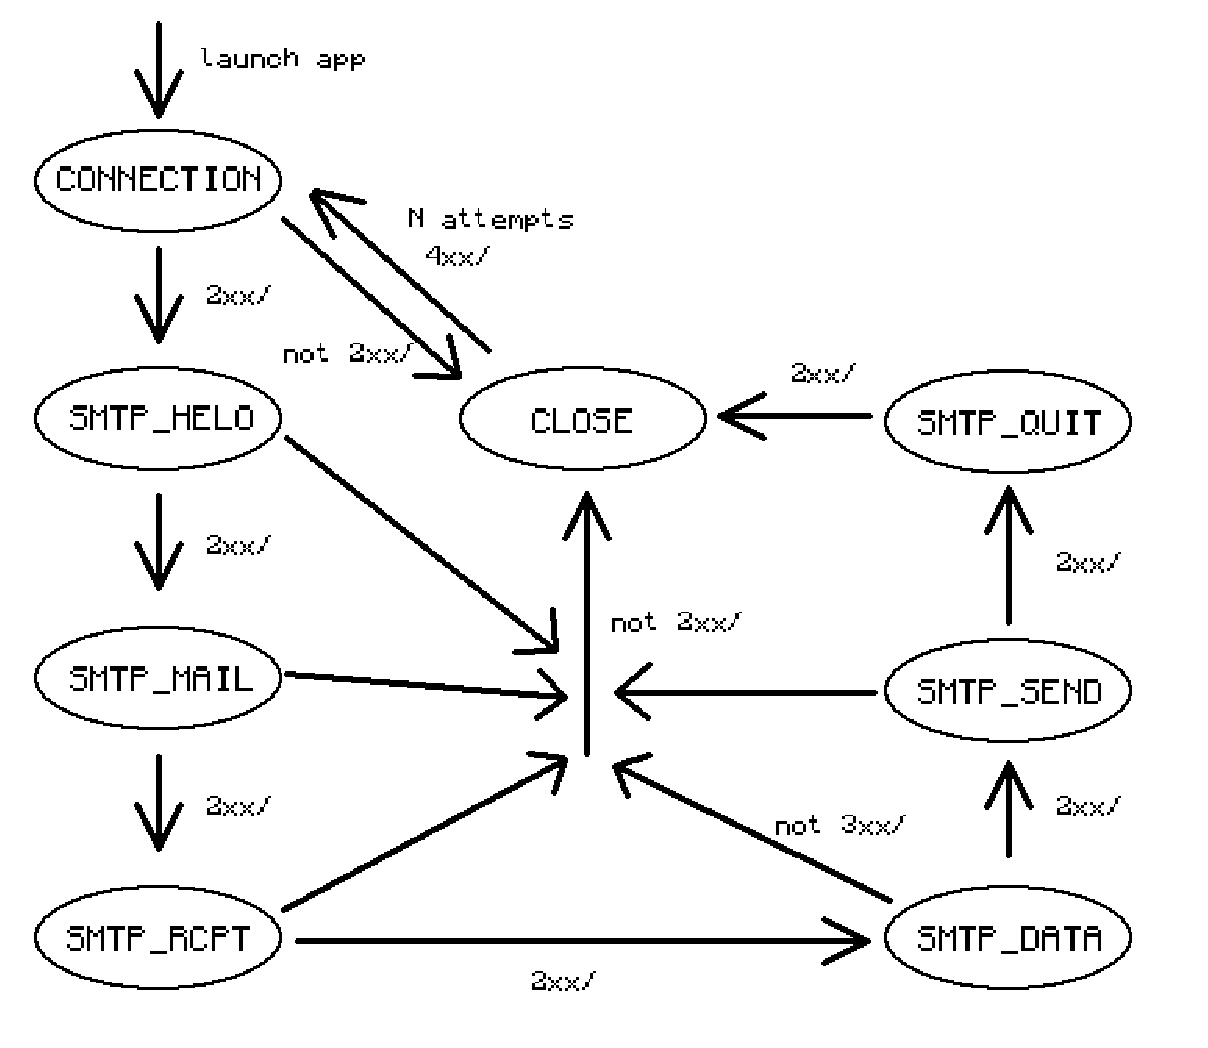
\includegraphics[width=0.95\textwidth]{State_Machine.pdf}
        \end{center}
        \caption{State Machine}\label{fig:}
    \end{figure}
    \subsection{Implementation}
    \subsubsection{Includes and Definitions}
    \begin{lstlisting}[language=C]
    #include <stdio.h>
    #include <unistd.h>
    #include <stdlib.h>
    #include <string.h>
    #include <netdb.h>
    #include <sys/types.h>
    #include <sys/socket.h>
    #include <sysexits.h>
    \end{lstlisting}
    \texttt{\#include} Directives: These include standard C libraries (\texttt{stdio.h}, \texttt{unistd.h}, \texttt{stdlib.h}, \texttt{string.h}, \texttt{netdb.h}, \texttt{sys/types.h}, \texttt{sys/socket.h}) and \texttt{sysexits.h} for exit status codes.
    \newpage

    \begin{lstlisting}[language=C]
    #define DEFAULT_PORT "25"
    #define MAX_ATTEMPTS 5
    #define WAIT_TIME 5
    \end{lstlisting}
    \textbf{Constants}
    \begin{itemize}
        \item \textbf{DEFAULT\_PORT}:  Default port number for SMTP (port 25)
        \item \textbf{MAX\_ATTEMPTS}: Maximum number of connection attempts
        \item \textbf{WAIT\_TIME}: Time to wait between connection attempts (in seconds)
    \end{itemize}

    \subsubsection{Function Declarations}
    \begin{lstlisting}[language=C]
    static FILE *tcp_connect(const char *hostname, const char *port);
    \end{lstlisting}
    \textbf{tcp\_connect} establishes a TCP connection to a specified hostname and port, returning a FILE* for socket communication.

    \subsubsection{SMTP State Machine}
    \begin{lstlisting}[language=C]
    typedef enum {
        CONNECTION,
        SMTP_HELO,
        SMTP_MAIL,
        SMTP_RCPT,
        SMTP_DATA,
        SMTP_SEND,
        SMTP_QUIT,
        CLOSE,
    } smtp_state_t;
    \end{lstlisting}
    Defines different states \textbf{(smtp\_state\_t)} for the SMTP client to manage the sequence of SMTP commands required to send an email

    \subsubsection{Main Function}
    \begin{lstlisting}[language=C]
    int main(int argc, char **argv)
    \end{lstlisting}
    Entry point of the program where command-line arguments are validated and SMTP communication is managed

    \subsubsection{Command Line Arguments}
    \begin{lstlisting}[language=C]
    if(argc < 6 || argc > 7) {
        fprintf(stderr, "[!] Usage: %s <sender email> <subject> <message file> <mail server> <receiver email> [<port>]\n", argv[0]);
        exit(EX_USAGE);
    }
    \end{lstlisting}
    \textbf{Argument Validation:} Ensures correct usage with necessary command-line arguments (sender email, subject, message file, mail server, receiver email, optional port)

    \subsubsection{Argument Parsing}
    \begin{lstlisting}[language=C]
    char *sender = argv[1];
    char *subject = argv[2];
    char *message_file = argv[3];
    char *mail_server = argv[4];
    char *receiver = argv[5];
    char *port = (argc == 7) ? argv[6] : DEFAULT_PORT;
    \end{lstlisting}
    \textbf{Argument Assignment:} Copies command-line arguments into variables for easier access and validation

    \subsubsection{File Handling}
    \begin{lstlisting}[language=C]
    FILE* mail_body = fopen(message_file, "r");
    if(mail_body == NULL) {
        fprintf(stderr, "[!] Could not open message file: %s\n", message_file);
        exit(EX_NOINPUT);
    }
    \end{lstlisting}
    \textbf{File Opening:} Opens the message file for reading. If the file cannot be opened, it exits with \textbf{EX\_NOINPUT}

    \subsubsection{SMTP Communication Loop}
    \begin{lstlisting}[language=C]
    smtp_state_t state = CONNECTION;
    // Loop to manage SMTP states and communication
    while(1) {
        switch(state) {
            // Each case handles a specific SMTP command/response sequence
        }
    }
    \end{lstlisting}
    \textbf{SMTP Communication Loop:} Continuously loops through SMTP states \textbf{(CONNECTION, SMTP\_HELO, SMTP\_MAIL, etc.)} to establish connection, send email data, and handle server responses

    \subsubsection{tcp\_connect Function}
    \begin{lstlisting}[language=C]
    static FILE *tcp_connect(const char *hostname, const char *port)
    \end{lstlisting}
    
    \section{Tests}
\end{document}
